%%%%%%%%%%%%%%%%%%%%%%%%%%%%%%%%%%%%%%%%%
% Plasmati Graduate CV
% LaTeX Template
% Version 1.0 (24/3/13)
%
% This template has been downloaded from:
% http://www.LaTeXTemplates.com
%
% Original author:
% Alessandro Plasmati (alessandro.plasmati@gmail.com)
%
% License:
% CC BY-NC-SA 3.0 (http://creativecommons.org/licenses/by-nc-sa/3.0/)
%
% Important note:
% This template needs to be compiled with XeLaTeX.
% The main document font is called Fontin and can be downloaded for free
% from here: http://www.exljbris.com/fontin.html
%
%%%%%%%%%%%%%%%%%%%%%%%%%%%%%%%%%%%%%%%%%

%----------------------------------------------------------------------------------------
%	PACKAGES AND OTHER DOCUMENT CONFIGURATIONS
%----------------------------------------------------------------------------------------

\documentclass[a4paper,10pt]{article} % Default font size and paper size

\usepackage{fontspec} % For loading fonts
\defaultfontfeatures{Mapping=tex-text}
\setmainfont[SmallCapsFont = Fontin SmallCaps]{Fontin} % Main document font

\usepackage{xunicode,xltxtra,url,parskip} % Formatting packages

\usepackage[usenames,dvipsnames]{xcolor} % Required for specifying custom colors

\usepackage[big]{layaureo} % Margin formatting of the A4 page, an alternative to layaureo can be \usepackage{fullpage}
% To reduce the height of the top margin uncomment: \addtolength{\voffset}{-1.3cm}

\usepackage{hyperref} % Required for adding links	and customizing them
\definecolor{linkcolour}{rgb}{0,0.2,0.6} % Link color
\hypersetup{colorlinks,breaklinks,urlcolor=linkcolour,linkcolor=linkcolour} % Set link colors throughout the document

\usepackage{titlesec} % Used to customize the \section command
\titleformat{\section}{\Large\scshape\raggedright}{}{0em}{}[\titlerule] % Text formatting of sections
\titlespacing{\section}{0pt}{3pt}{3pt} % Spacing around sections

\usepackage{multicol}

\begin{document}

\pagestyle{empty} % Removes page numbering

\font\fb=''[cmr10]'' % Change the font of the \LaTeX command under the skills section

%----------------------------------------------------------------------------------------
%	NAME AND CONTACT INFORMATION
%----------------------------------------------------------------------------------------

\par{\centering{\Huge Damien Michael \textsc{Carver}}\bigskip\par}
%\par{\centering \footnotesize Young graduate willing to start his career in \emph{High Performance Computing} \par}
%\par{\centering \footnotesize Young graduate willing to do a PhD Thesis in C.S. \par}
\par{\centering \footnotesize First year PhD student in C.S. \par}

\section{Personal Data}

\begin{tabular}{rl}
	\textsc{Nationality and Date of Birth:} & Mauritian  | 22 May 1991 \\
	%\textsc{Address:} & 38 Rue Yves Le Coz 78000 Versailles, France\\
	\textsc{Address:} & 150 Faubourg Saint-Antoine 75012 Paris, France\\
	\textsc{Phone:} & +33 6 73 14 99 89\\
	\textsc{email:} & \href{carverdamien@gmail.com}{carverdamien@gmail.com}
\end{tabular}

%----------------------------------------------------------------------------------------
%	WORK EXPERIENCE 
%----------------------------------------------------------------------------------------

\section{Work Experience}

\begin{tabular}{r|p{11cm}}
%------------------------------------------------

\textsc{April 2015} & PhD Student at \textsc{LIP6 INRIA}, Paris\\
\textsc{Currently} & \footnotesize{
						Working on linux kernel cgroup memory subsystem.
					}\\
\multicolumn{2}{c}{} \\

%------------------------------------------------

\textsc{Dec 2014} & Software Engineer at \textsc{Magency Digital}, Paris\\
\textsc{Currently} & \footnotesize{
						Moving Magency's infrastructure towards Container Virtualization.
					}\\
\multicolumn{2}{c}{} \\

%------------------------------------------------

\textsc{Apr 2014} & Intern at \textsc{TOTAL E\&P R\&T}, Houston\\
\textsc{Aug 2014} & \footnotesize{
						Prototyped an I/O scheduling algorithm using \emph{Graph of Tasks Programming Models} and contributed to software development.
					}\\
\multicolumn{2}{c}{} \\

%------------------------------------------------

\textsc{Jun 2013} & Summer Intern at \textsc{LIP6}, Paris\\
\textsc{Jul 2013} & \footnotesize{
						Prototyped a parallel and concurrent SAT solver.
					}\\
\multicolumn{2}{c}{} \\

%------------------------------------------------
\end{tabular}

%----------------------------------------------------------------------------------------
%	EDUCATION
%----------------------------------------------------------------------------------------

\section{Education}

\begin{tabular}{rl}

%------------------------------------------------

\textsc{Sep 2012} & M.S. in \textsc{Computer Science}, \textbf{University of Pierre and Marie Currie}, Paris\\
\textsc{Aug 2014} & Major: \emph{Distributed Systems and Applications}\\
                  & \normalsize \textsc{Good Grade} \hyperlink{grds_ms}{\hfill | \footnotesize Detailed List of Courses}\\
&\\

%------------------------------------------------

\textsc{Sep 2009} & B.S. in \textsc{Computer Science}, \textbf{University of Pierre and Marie Currie}, Paris \\
\textsc{Aug 2012} & Majors: \emph{Computer Science} and \emph{Applied Mathematics}\\
				  & \normalsize \textsc{Good Grade} \hyperlink{grds_bs}{\hfill| \footnotesize Detailed List of Courses}\\
&\\

%------------------------------------------------

\textsc{Jul 2011} & Exchange Courses at \textbf{Brown University}, Providence\\
&\\

%------------------------------------------------

\textsc{Jun 2009} & Scientific Baccalaur\'eat, Mauritius | Very Good Grade %: 16/20

%------------------------------------------------

\end{tabular}

%----------------------------------------------------------------------------------------
%	SCHOLARSHIPS AND ADDITIONAL INFO
%----------------------------------------------------------------------------------------

% \section{Scholarships and Certificates}

% \begin{tabular}{rl}
% \textsc{Sept.} 2012 & Faculty of Science Masters Scholarship \footnotesize(\$30,000)\normalsize\\

% \textsc{June} 2010 & {\textsc{Gmat}\textregistered}\setmainfont[SmallCapsFont=Fontin SmallCaps]{Fontin-Regular}: 730 (\textsc{q:50;v:39}) 96\textsuperscript{th} percentile; \textsc{awa}: 6.0/6.0 (89\textsuperscript{th} percentile)
% \end{tabular}

%----------------------------------------------------------------------------------------
%	LANGUAGES
%----------------------------------------------------------------------------------------

\section{Languages}

\begin{tabular}{rlrl}
\textsc{English:}   & Fluent, \href{http://www.certification-cles.fr}{CLES B2}\\
\end{tabular}
\hfill
\begin{tabular}{rl}
\textsc{French:}    & Mother tongue\\
\end{tabular}

%----------------------------------------------------------------------------------------
%	COMPUTER SKILLS 
%----------------------------------------------------------------------------------------

\section{Technical Skills}

\begin{tabular}{rl}
Languages :                         & C/C++, Fortran, Java, Objective-C       \\
Programming Models :                & MPI, OpenMP, CUDA, OmpSs, CnC           \\
%Middlewares :                       & Hadoop, CORBA, RMI, RPC                 \\
Script Languages :                  & bash, pyhton, perl                      \\
Tools :                             & docker, git, \LaTeX, gnuplot, makefile   \\
%Mathematical Tools :                & Matlab, Scilab, Mathematica             \\
\end{tabular}

%----------------------------------------------------------------------------------------
%	INTERESTS AND ACTIVITIES
%----------------------------------------------------------------------------------------

\section{Interests and Activities}

Roller Skating, Running, Hiking, Cooking and Japanese Language.

%----------------------------------------------------------------------------------------

\newpage

%----------------------------------------------------------------------------------------
%	GRADE TABLES
%----------------------------------------------------------------------------------------

\par{\centering\Large \hypertarget{grds_ms}{Master of Science in \textsc{Computer Science}}\par}
\large{\centering Grades\par}\normalsize

\begin{center}
\begin{tabular}{lcc}
\multicolumn{1}{c}{\textsc{Course}} & \textsc{Grade}&\textsc{Credit Hrs}\\
\hline
Final Internship                                           &       77,5/100 & 18    \\
Research Group : Distributed Applications                  &       70/100 & 3     \\
Research Group : Informatics Systems                       &       85/100 & 3     \\
Engineering Group : Embedded Systems                       &   80/100 & 3     \\
Engineering Group : Distributed Systems                    &     62,5/100   & 3     \\
\hline
Advanced Distributed Algorithms                            &  75,1/100 & 3     \\
Advanced Parallel Programming                              &    87/100 & 3     \\
Automated Production of Distributed Applications           &  72,5/100 & 3     \\
Formal Verification of Distributed Systems                 &  67,5/100 & 3     \\
Mobile Device Programming                                  &  62,1/100 & 3     \\
Foundation of Real-Time Embedded Systems                   &   100/100 & 3     \\
Platforms for Advanced Informatics Systems                 &  75,1/100 & 3     \\
Parallel Programming                                       &    77/100 & 3     \\
Multi-core Kernels and Virtualization                      &  88,5/100 & 3     \\
Environments for Embedded or Real-Time Distributed Systems &  67,5/100 & 3     \\
\hline
Project : Kernel Placement Algorithm                       & 93,75/100 & 6     \\
Distributed Databases                                      & 83,85/100 & 6     \\
Distributed Algorithms                                     &    67/100 & 6     \\
English                                                    & 79,25/100 & 6     \\
Client/Server Distributed Systems                          &  95,1/100 & 6     \\
Networks and System Administration                         &  91,5/100 & 6 \\
\hline
OS Kernel's Advanced Architecture                          &  89,5/100 & 6     \\
Processor's Architecture and Optimisations                 &    54/100 & 6     \\
POSIX Advanced Programming                                 &  70,5/100 & 6     \\
Software Engineering                                       &    82/100 & 6     \\
Networks' Architecture	                                   &    64/100 & 6     \\
Advanced Algorithmic                                       &    85/100 & 6 \\
\hline
\end{tabular}
%{\footnotesize N/A* Not yet available}
\end{center}
\bigskip
\bigskip

%------------------------------------------------

\newpage

\par{\centering\Large \hypertarget{grds_bs}{Bachelor of Science in \textsc{Computer Science and Applied Mathematics}}\par}\large{\centering Grades\par}\normalsize

\begin{center}
\begin{tabular}{lcc}
\multicolumn{1}{c}{\textsc{Course}} & \textsc{Grade} & \textsc{Grade Points}\\
\hline
\textsc{2011 - 2012} & & \\
\hline
Introduction to Numerical Imaging                          &  77,5/100 & 6     \\
Introduction to Cryptology                                 &   100/100 & 6     \\
Models for Optimization and Decision                       &  62,5/100 & 6     \\
Numerical Methods for differential equations               & 65,94/100 & 6     \\
Bioinformatics                                             &    65/100 & 3     \\
English                                                    &    71/100 & 3     \\
\hline
Object-oriented Programming                                &  87,5/100 & 6     \\
Algorithm Analysis and Conception                          & 80,63/100 & 6     \\
Introduction to Numerical Analysis                         &    49/100 & 6     \\
Probability                                                &    67/100 & 6     \\
Introduction to Topology and Calculus                      &    88/100 & 6     \\
English                                                    &  72,5/100 & 3     \\
\hline
\textsc{2010 - 2011} & & \\
\hline
Brown Exchange : Introduction to Machine Learning          &    70/100 & 6     \\
Analysis and Algebra                                       &    77/100 & 3     \\
Multi-variable functions and multi-integrals               & 85,25/100 & 6     \\
English                                                    &    84/100 & 3     \\
\hline
Geometry and Algebra                                       &    53/100 & 12    \\
Introduction to System multiprogramming                    &  82,1/100 & 6     \\
Scientific Computation                                     &    70/100 & 6     \\
Algorithmic                                                &  72,5/100 & 6     \\
\hline
Imperative Programming and Data Structure in C             & 90,74/100 & 6     \\
Introduction to Tasks Automation                           & 58,88/100 & 6     \\
Arithmetic                                                 &    63/100 & 6     \\
Series and Integrals                                       &  65,5/100 & 12    \\
\hline
\end{tabular}
\end{center}

%----------------------------------------------------------------------------------------

\newpage

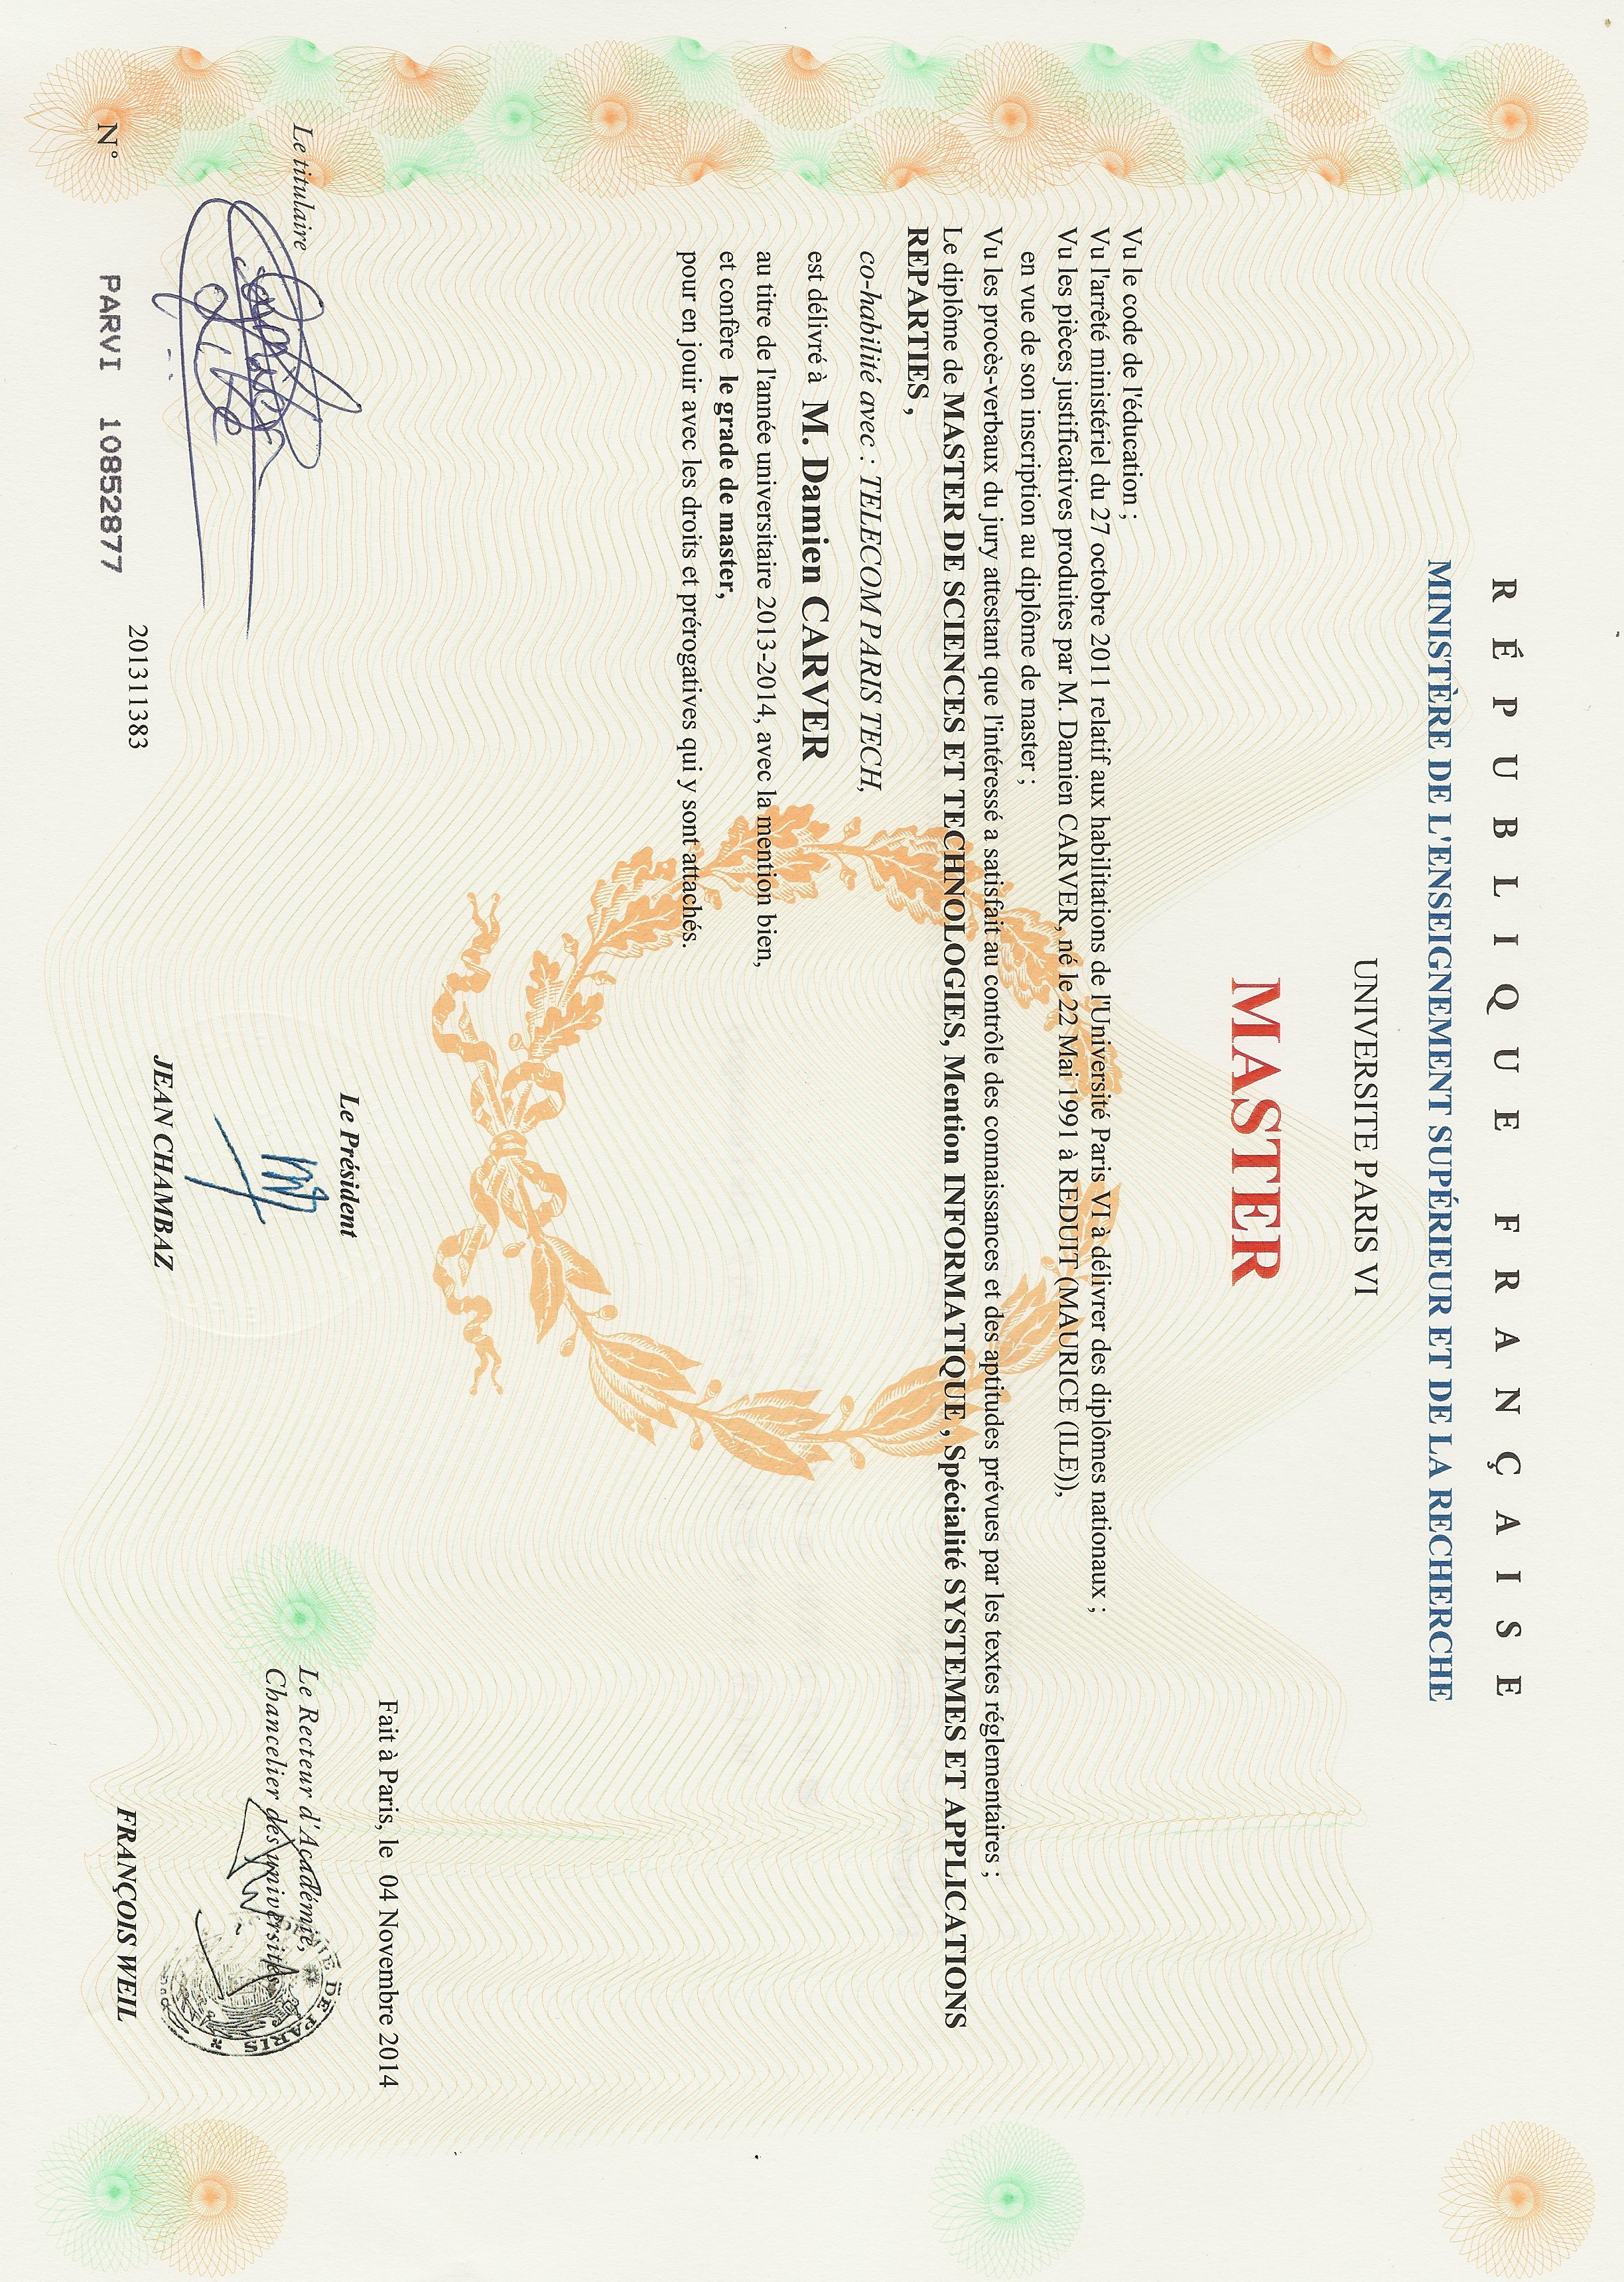
\includegraphics[scale=0.7]{./m2.jpeg}

%----------------------------------------------------------------------------------------

\end{document}
